\section{Introduction} 
    Concurrent programs take advantage of \textit{out-of-order} execution. Intuitively, this means that more than one unrelated computations can be done ``simultaneously'' without having any fixed order in which they should happen. 
    This results in concurrent programs having multiple different outcomes, the possible outcomes of which are described by
    a \textit{memory consistency model}. 
    The most intuitive and commonly relied upon model is that of \textit{Sequential Consistency} (SC), which guarantees that every outcome of a program must be equivalent to a sequential interleaving of each thread's individual actions. 
    For example, consider the program in Figure~\ref{intro:Example} with two threads, which share memory denoted by $x$, $y$ initialized to 0, where $a$, $b$ are local variables. The right-hand-side are the possible values that $a$ and $b$ can read under sequential consistency rules.
    
    %Show program 
    \begin{figure}[H]
        \centering
        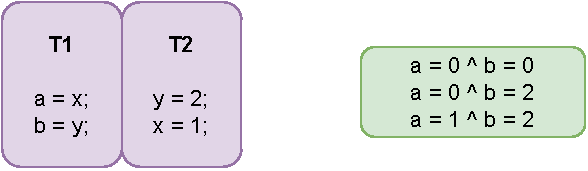
\includegraphics[scale=0.7]{Program_Example.pdf}
        \caption{Example program with its possible outcomes under sequential consistency.}
        \label{intro:Example}
    \end{figure}
    
    
    However, the above program under SC cannot have the outcome $a=2\ \wedge\ b=0$. 
    From a program transformation standpoint, such an outcome should be possible: we can simply reorder either both the reads or both writes to $x$ and $y$, as they are computations on disjoint memory. 
    But from a consistency rule standpoint, since the outcome is not valid, it also brings with it the conclusion that such simple program transformations may not be safe or even invalid.
    Figure~\ref{intro:Example2} shows how after doing either one of these reorderings, an outcome invalid under SC is possible. 
    %Show program 
    \begin{figure}[H]
        \centering
        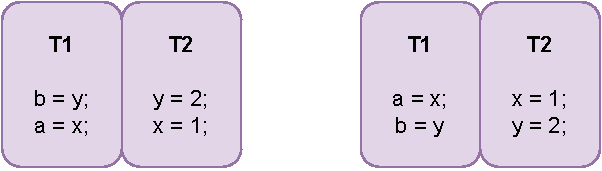
\includegraphics[scale=0.7]{Program_Transform_Example.pdf}
        \caption{Left program is when the two reads in T1 are reordered, whereas the right program is when the two writes of T2 are reordered.}
        \label{intro:Example2}
    \end{figure}
    
    %Should I also state here that we cannot use the hardware features??
    
    Weaker consistency models have been introduced to concurrent, shared-memory languages to leverage more of the \textit{}{out-of-order} notion. 
    For instance,  under the ECMAScript consistency model semantics, if all the accesses are of type \textit{unordered}, the above invalid outcome is allowed, which implies a reordering of such events is valid in the above case. 
    The problem though is that semantics of such weak consistency can be easily misunderstood, and is sometimes defined in informal prose format, thus leading to misinterpretation of intended semantics, which leads to implementation issues. 
    The lack of clear semantics also makes it difficult to assert when a particular program transformation is valid / safe (in our case, instruction reordering).
    
    Our focus in this work is to offer a clarified, more concise rendition of the core ECMAScript memory model that allows for better abstract reasoning over allowed and disallowed behaviours (outcomes). 
    We use our model to provide a straightforward, conservative proof of when reordering of independent instructions is permitted, addressing optimization in terms of its impact on observable program behaviours. 
    Our approach can be extended to address additional optimization effects, such as redundancy removal. Specific contributions of our work include the following:
    
    \begin{enumerate}
        \item We provide a concise \textit{declarative style} model of the core ECMAScript memory consistency semantics. This clarifies the existing draft presentation~\cite{ECMA} in a manner useful for validating optimizations.
        \item Using our model we show when basic reordering of independent instructions is allowed. Although conservative, this represents a formal proof that this fundamental optimization is permitted. Similar proof designs can be used to validate other basic optimization behaviours,such as removing redundant reads or writes.
    \end{enumerate}
  